% ============================================================
%  proposal-main.tex
%  Amrita Vishwa Vidyapeetham – Thesis PROPOSAL driver
%  ============================================================
%  Use this file instead of main.tex when writing a Thesis
%  Proposal (pre-qualifying / open seminar document).
%  It uses the article class (no chapters) to match the
%  format used in the sample proposal.
%
%  Compile:  pdflatex proposal-main  →  bibtex proposal-main
%            →  pdflatex proposal-main  →  pdflatex proposal-main
% ============================================================

\documentclass[12pt,a4paper]{article}
\renewcommand{\refname}{References}
% ---- Load personal / document information ------------------
\newcommand{\DocType}{proposal}
% ============================================================
%  doc-info.tex
%  Amrita Vishwa Vidyapeetham – Doctoral Document Template
%  ============================================================
%  INSTRUCTIONS:
%  Edit ONLY this file to customise your document.
%  All front matter (title page, certificate, abstract, etc.)
%  reads its content from the macros defined here.
% ============================================================

%% ---- Scholar information -----------------------------------
\newcommand{\AuthorName}{Siju K.S}
\newcommand{\AuthorRegNo}{CB.AI.R4CEN24003}
\newcommand{\AuthorDegree}{Doctor of Philosophy}

% ---- Thesis / proposal title --------------------------------
\newcommand{\DocTitle}{Advanced Deep Learning Architectures and
  Adaptive Frameworks for Medical Image Restoration}
% ---- Abstract keywords -------------------------------------
\newcommand{\AbstractKeywords}{Medical image restoration, deep learning,
	chest X-ray denoising, image deblurring, generative adversarial network,
	activation function, test-time refinement, Sobolev loss, edge preservation}
% ---- Supervisors -------------------------------------------
\newcommand{\SupervisorName}{Dr.~Vipin V}
\newcommand{\SupervisorDesignation}{Associate Professor}
\newcommand{\SupervisorDept}{Department of Artificial Intelligence}
\newcommand{\SupervisorCampus}{Amrita Vishwa Vidyapeetham, Coimbatore Campus}

\newcommand{\CoSupervisorName}{Dr.~Mithun Kumar Kar}
\newcommand{\CoSupervisorDesignation}{Assistant Professor}
\newcommand{\CoSupervisorDept}{Department of Artificial Intelligence}
\newcommand{\CoSupervisorCampus}{Amrita Vishwa Vidyapeetham, Coimbatore Campus}

% ---- Department / Faculty ----------------------------------
\newcommand{\DeptName}{Artificial Intelligence}
\newcommand{\FacultyName}{Faculty of Artificial Intelligence}
\newcommand{\CampusName}{Coimbatore Campus (India)}
\newcommand{\UniversityName}{Amrita Vishwa Vidyapeetham}

% ---- Head of Department / Dean (for certificate) ----------
\newcommand{\HODName}{Dr.~[HOD Name]}
\newcommand{\HODDesignation}{Head of the Department}
\newcommand{\DeanName}{Dr.~[Dean Name]}
\newcommand{\DeanDesignation}{Dean, Faculty of Engineering \& Technology}

% ---- Submission details ------------------------------------
\newcommand{\SubmissionMonth}{May}
\newcommand{\SubmissionYear}{2026}
\newcommand{\SubmissionDate}{\SubmissionMonth~\SubmissionYear}
% ---- School name (as it appears on certificate/declaration) ----
\newcommand{\SchoolName}{Amrita School of Engineering}

% ---- Thesis defense / submission date for declaration ----------
\newcommand{\ThesisDefenseDate}{~~~~~~~~~~~~~~~~~~~~~~~~~~}   % fill in before submission

% ---- Partial-fulfilment phrase (auto-set by DocType) -------
% Override here only if your department uses different wording.
\newcommand{\FulfilmentPhrase}{%
  Submitted in partial fulfilment of the requirements for the\\
  award of the Degree of \AuthorDegree\\
  under the \FacultyName}

% ---- Logo path (relative to main .tex file) ----------------
\newcommand{\UniversityLogoPath}{images/amrita-logo.png}

% ---- Dedication (leave blank to suppress dedication page) --
\newcommand{\DedicationText}{%
  \textit{To my parents, family, and teachers,\\
  whose guidance and blessings made this journey possible.}}

% ---- Acknowledgements text ---------------------------------
% Write your acknowledgements in frontmatter/acknowledgements.tex
% (this macro is unused but kept for reference)
\newcommand{\AcknowledgementsFile}{frontmatter/acknowledgements.tex}


% ---- Conditional inclusion helper --------------------------
\usepackage{ifthen}
\usepackage{lipsum}
% ---- Load global configuration (only the article-compatible subset)
\usepackage[
  a4paper,
  top    = 1.0in,
  bottom = 1.0in,
  left   = 1.25in,
  right  = 1.0in
]{geometry}
\usepackage[utf8]{inputenc}
\usepackage[T1]{fontenc}
\usepackage{times}
\usepackage{setspace}
\onehalfspacing
\usepackage{amsmath,amssymb}
\usepackage{graphicx}
\graphicspath{{images/}}
\usepackage{float}
\usepackage{caption}
\usepackage{subcaption}
\usepackage{booktabs}
\usepackage{multirow}
\usepackage{longtable}
\usepackage{natbib}
\bibliographystyle{plainnat}
\usepackage[
  colorlinks = true,
  citecolor  = blue,
  linkcolor  = black,
  urlcolor   = blue
]{hyperref}
\usepackage{url}
\usepackage{enumitem}
\usepackage{ifthen}

% Section formatting (Amrita style – article class)
\usepackage{titlesec}
\titleformat{\section}{\large\bfseries}{\thesection}{1em}{}
\titleformat{\subsection}{\normalsize\bfseries}{\thesubsection}{1em}{}
\titleformat{\subsubsection}{\normalsize\bfseries}{\thesubsubsection}{1em}{}

\newcommand{\HRule}{\rule{\linewidth}{0.5mm}}
\newcommand{\signaturebox}[2]{%
  \begin{tabular}{@{}l@{}}
    \rule{5.5cm}{0.4pt}\\
    \textbf{#1}\\
    #2
  \end{tabular}}

% ============================================================
\begin{document}
% ============================================================

% ---- TITLE PAGE ----
\pagenumbering{gobble}
\begin{titlepage}
  \centering
  \vspace*{0.5cm}
  {\Large\bfseries \DocTitle \par}
  \vspace{1.2cm}
  {\large\bfseries Thesis Proposal \par}
  \vspace{1cm}
  Submitted in partial fulfilment of the Degree of \\
  \AuthorDegree\ under the \\
  \FacultyName \\
  \vspace{1cm}
  \textit{by}\\[0.5cm]
  {\large\bfseries \AuthorName}\\
  {\large \AuthorRegNo}
  \vspace{1cm}

  \textit{Under the guidance of}\\[0.5cm]
  {\large\bfseries\itshape \SupervisorName \\[0.2cm] \CoSupervisorName}

  \vfill
  \IfFileExists{\UniversityLogoPath}{%
    \includegraphics[width=0.45\textwidth]{\UniversityLogoPath}\\[1cm]}{%
    \textbf{[Insert university logo]}\\[1cm]}

  {\large\bfseries Department of \DeptName}\\[0.1cm]
  {\large\bfseries \MakeUppercase{\UniversityName}}\\[0.1cm]
  {\large\bfseries \MakeUppercase{\CampusName}}\\
  \vspace{1cm}
  {\large \SubmissionDate}
\end{titlepage}

% ---- FRONT MATTER ------------------------------------------
\pagenumbering{roman}
\tableofcontents
\newpage
\pagenumbering{arabic}

% ---- PROPOSAL SECTIONS -------------------------------------
% Each section is a separate file in the chapters/ folder.
% Rename or add sections to match your proposal structure.

% chapters/proposal-abstract.tex
\section*{Abstract}
\addcontentsline{toc}{section}{Abstract}

Medical images acquired using X-ray and computed tomography (CT) are often degraded by acquisition noise and patient motion. This reduces diagnostic accuracy. Deep learning (DL) methods have shown promise for image restoration, but existing approaches have limitations. Standard denoisers often smooth out fine anatomical details. Most activation functions (AFs) apply the same operation everywhere, without considering local context. Even models that incorporate physics during training may leave residual artefacts because training minimises average error over a dataset, not per-image quality.

This thesis addresses these limitations through a three-phase investigation.

In Phase I, we developed X-GAN, a physics-informed generative adversarial network for chest X-ray denoising. X-GAN uses a U-Net generator with an edge attention mechanism that explicitly preserves anatomical boundaries. A hybrid loss function combines pixel fidelity, edge preservation, and structural similarity. X-GAN achieves a peak signal-to-noise ratio (PSNR) of 36.48 dB and an edge preservation index (EPI) of 0.721 with only 2.17 million parameters. In a downstream diagnostic task, denoising with X-GAN improved ResNet-50 accuracy from 54.55\% to 79.52\%.

In Phase II, we proposed SAGA, a spatially adaptive gated AF for medical image deblurring. Unlike standard AFs such as Rectified Linear Units (ReLU), SAGA computes its output based on local spatial context. It uses a learnable gating mechanism to decide where to sharpen edges and where to suppress noise. SAGA outperforms six existing AFs across four different network architectures. On average, it improves PSNR by 6.3 dB and structural similarity (SSIM) by 0.09 over ReLU. Layer-wise relevance propagation shows that SAGA focuses network attention on diagnostically relevant boundaries.

In Phase III, we plan to develop a test-time refinement framework called Viveka and a Sobolev-regularised loss function called augmented differential L1  (ADL\(_1\)) with an attention-guided U-Net (AG-UNet). Viveka will apply physics-based constraints directly at inference time. It will use frequency-domain detail extraction, anatomically adaptive gains based on X-ray attenuation coefficients, and uncertainty-weighted edge protection. Viveka will be model-agnostic and will process images in under one second on a standard CPU. The ADL\(_1\) loss will explicitly penalise gradient errors, providing mathematical guarantees on edge preservation. The AG-UNet architecture will use gradient-guided skip connections to preserve fine structural details. Preliminary experiments indicate that this framework can recover trabecular bone texture that standard losses erase.

Collectively, this research bridges the gap between algorithmic performance and clinical reliability. It delivers a framework that is physics-aware, interpretable, and ready for real-world deployment.

\noindent\textbf{Keywords:} keyword1, keyword2, keyword3.

\newpage
% chapters/proposal-introduction.tex
% Replace the content below with your own text.

\section{Introduction}
\label{sec:introduction}

Medical imaging is essential for modern diagnosis, treatment planning, and disease monitoring. X-ray and computed tomography (CT) are the most widely used modalities because they are fast, accessible, and cost-effective. In low-income countries with limited access to MRI or ultrasound, X-ray remains the primary diagnostic tool for conditions ranging from fractures to pneumonia.

However, image quality is often degraded during acquisition. This reduces diagnostic accuracy and can lead to missed findings, false positives, or unnecessary repeat scans. Poor image quality also forces clinicians to request additional views or higher radiation doses, increasing patient risk.

The two main types of degradation are quantum noise and motion blur.

Quantum noise occurs in low-dose X-ray protocols. When the number of photons reaching the detector is limited, random fluctuations appear. These fluctuations follow a Poisson distribution. The noise is signal-dependent: dense structures such as bone suffer more relative noise than soft tissue. This is why bone edges often appear grainy in low-dose chest X-rays.

Motion blur occurs when patients breathe, their hearts beat, or they move involuntarily. This creates spatially varying blur that reduces the sharpness of anatomical boundaries. In chest CT, breathing motion can create streak artefacts that obscure lung nodules.

Classical restoration methods such as Wiener filtering and total variation regularisation attempt to reverse these degradations. They assume that blur is uniform across the image and that noise follows a simple statistical model. These assumptions fail in medical imaging, where motion creates complex, non-uniform patterns and quantum noise is signal-dependent.

Deep learning (DL) methods have become the standard for image restoration. U-Net and ResNet architectures learn to map degraded inputs to clean outputs directly from data. For denoising, models such as DnCNN \citep{zhang2017beyond}, RIDNet \citep{anwar2019real}, CBDNet \citep{guo2019toward}, and X-ReCNN \citep{jin2019chest} have been proposed. For deblurring, models such as DeblurGAN~\citep{kupyn2019deblurgan} and multi-scale convolutional networks have been developed.

However, DL methods have their own limitations.

First, standard loss functions such as mean absolute error minimise pixel-wise differences but do not explicitly preserve edges. As a result, denoised images often appear smooth and waxy, with fine details such as bone trabeculae and lung markings erased.

Second, most activation function (AFs) such as Rectified Linear Units (ReLU) apply the same non-linearity to every spatial location~\citep{nair2010rectified}. They cannot distinguish between anatomical edges that should be preserved and noise that should be suppressed.

Third, even models that incorporate physics during training are optimised for average performance over a dataset. A model that works well on average may still produce visible artefacts on a specific patient image.

Fourth, standard loss functions provide no control over gradient fidelity. We formally prove this as the Sobolev Gap: a network can achieve arbitrarily low pixel error while having arbitrarily large gradient errors.

This thesis addresses these limitations through a three-phase investigation.

In Phase I, we developed X-GAN, a physics-informed generative adversarial network for chest X-ray denoising~\citep{siju2026xgan}. X-GAN uses a U-Net ~\citep{ronneberger2015unet} generator with an edge attention mechanism that explicitly preserves anatomical boundaries. A hybrid loss function combines pixel fidelity, edge preservation, and structural similarity. X-GAN achieves a peak signal-to-noise ratio of 36.48 dB and an edge preservation index of 0.721 with only 2.17 million parameters.

In Phase II, we proposed SAGA, a spatially adaptive gated AF for medical image deblurring~\citep{siju2026saga}. Unlike standard AFs such as ReLU, SAGA computes its output based on local spatial context. It uses a learnable gating mechanism to decide where to sharpen edges and where to suppress noise. SAGA outperforms six existing AFs across four network architectures, improving PSNR by 6.3 dB on average over ReLU.

In Phase III, we plan to develop a test-time refinement framework called Viveka and a Sobolev-regularised loss function called ADL\(_1\) with an attention-guided U-Net architecture. Viveka will apply physics-based constraints directly at inference time without modifying network weights. The ADL\(_1\) loss will provide mathematical guarantees on edge preservation.

The remainder of this thesis proposal is organised as follows. Section~\ref{sec:bs} presents background study and Section \ref{sec:lr} provides the details of literature review. Section~\ref{sec:rg} identifies research gaps and states the problem. Section~\ref{sec:rq} lists problem statements. Section~\ref{sec:ro} describes research objectives. Sections~\ref{sec:xgan} and \ref{sec:saga} present completed work on X-GAN and SAGA. Section~\ref{sec:phase3} describes planned work on Viveka and ADL\(_1\). Sections~\ref{sec:ec} to \ref{sec:cp} present expected contributions, publications, and completion plan.
% chapters/proposal-background.tex
% Replace the content below with your own text.

\section{Background}
\label{sec:background}

% Your content here.\section{Background Study}
\label{sec:bs}

\subsection{Physics of X-ray imaging}

The formation of an X-ray image follows the Beer-Lambert law \citep{bushberg2011essential}. The intensity at the detector is given by:

\[
I(x) = I_0 \exp\left(-\int_0^L \mu(s,x) ds\right)
\]

where \(\mu(s,x)\) is the spatially varying attenuation coefficient. Different tissues attenuate X-rays differently. Bone, with an attenuation coefficient of approximately 0.3 to 0.5 cm\(^{-1}\) at diagnostic energies, creates sharp intensity discontinuities. Lung parenchyma, with an attenuation coefficient of approximately 0.02 to 0.05 cm\(^{-1}\), requires moderate enhancement to reveal fine vasculature \citep{bushberg2011essential}. Background regions, where attenuation is negligible, contain only quantum noise.

Photon arrival follows a Poisson distribution, making the noise signal-dependent \citep{maier2018medical}. The observed intensity \(I_{\text{obs}}\) is a random variable:

\[
P(I_{\text{obs}}(x) | I(x)) = \frac{(I(x))^{I_{\text{obs}}(x)} \exp(-I(x))}{I_{\text{obs}}(x)!}
\]

The signal-to-noise ratio is proportional to \(\sqrt{I(x)}\), meaning dense structures such as bone suffer proportionally more relative noise than soft tissue \citep{bushberg2011essential}. This is why denoising chest X-rays is particularly challenging in bone-rich regions, as addressed by our X-GAN work \citep{siju2026xgan}.

\subsection{Physics of CT}

CT imaging acquires X-ray projections from multiple angles around the patient. The sinogram \(p(\theta, r)\) records the line integrals of attenuation coefficients \citep{bushberg2011essential}:

\[
p(\theta, r) = \int_{-\infty}^{\infty} \mu(x, y) ds
\]

where \(\theta\) is the projection angle and \(r\) is the detector position. The image is reconstructed using filtered back-projection or iterative methods \citep{maier2018medical}. Noise in CT follows a similar Poisson-Gaussian mixture as X-ray, but the reconstruction process can amplify noise and create streak artefacts \citep{jin2017deep}.

For our CT experiments, we used chest CT scans from public datasets \citep{syed2024medical}. The degradation in CT images is typically caused by patient motion during breath-holding or cardiac pulsation, creating motion blur that is spatially varying. This forms the basis for evaluating our SAGA AF \citep{siju2026saga} and the planned ADL\(_1\) loss.

\subsection{Physics of dual-energy X-ray absorptiometry (DXA)}

DXA is used for osteoporosis assessment. Two X-ray energies (typically 40 keV and 80 keV) are used to separate bone and soft tissue \citep{bushberg2011essential}. The bone mineral density is calculated from the attenuation ratios. DXA images contain sparse, high-frequency trabecular bone structures against a dark background \citep{wani2021knee}. This modality is challenging for deblurring because the diagnostic information is carried by fine bone struts that are easily smoothed by standard denoising methods, a problem addressed by our SAGA work \citep{siju2026saga} and the planned AG-UNet architecture.

\subsection{Image degradation models}

In medical imaging, the observed degraded image \(y\) is modelled as \citep{jin2017deep}:

\[
y = k * x + n
\]

where \(x\) is the clean image, \(k\) is a blur kernel, \(*\) denotes convolution, and \(n\) is additive noise.

For our experiments, we used three types of blur to simulate realistic acquisition artefacts \citep{nah2017deep, kupyn2019deblurgan}:

\noindent\textbf{Gaussian blur:} Models sensor noise and optical imperfections. The kernel is defined as:

\[
k_{\text{Gaussian}}(u,v) = \frac{1}{2\pi\sigma^2} \exp\left(-\frac{u^2 + v^2}{2\sigma^2}\right)
\]

We used \(\sigma\) values from 1.0 to 5.0 pixels.

\noindent\textbf{Motion blur:} Models patient movement during acquisition. The kernel is a line segment of length \(L\) pixels at angle \(\theta\). We used kernel lengths 9, 15, and 21 pixels.

\noindent\textbf{Defocus blur:} Models images captured outside the focal plane. The kernel is a disk of radius \(r\). We used radii from 2 to 5 pixels.

For denoising, we used Poisson noise to simulate low-dose acquisitions \citep{siju2026xgan}:

\[
I_{\text{noisy}} \sim \text{Poisson}(\lambda \cdot I_{\text{clean}})
\]

where \(\lambda\) is the peak photon parameter set to 1000 in our X-GAN and Viveka experiments \citep{siju2026xgan}.

\subsection{Sobolev spaces for image restoration}

The Sobolev space \(W^{1,1}(\Omega)\) couples pixel intensity with local geometry through the norm \citep{adams2003sobolev, evans2010partial}:

\[
\|u\|_{W^{1,1}(\Omega)} = \|u\|_{L^1(\Omega)} + \|\nabla u\|_{L^1(\Omega)}
\]

The first term ensures intensity fidelity by matching global tissue density. The second term, defined as the integral of the gradient magnitude, enforces structural fidelity by quantifying the cumulative sharpness of spatial transitions. This is equivalent to total variation \citep{rudin1992nonlinear}.

A key theoretical result is that the embedding \(L^1(\Omega) \hookrightarrow W^{1,1}(\Omega)\) is not continuous \citep{adams2003sobolev}. This means convergence in pixel intensity does not guarantee convergence in gradients. A network can achieve arbitrarily low MAE while having arbitrarily large gradient errors. We call this the Sobolev Gap, which we formally prove in our ADL\(_1\) work. This observation motivates the need for loss functions that explicitly constrain gradients, such as the ADL\(_1\) loss proposed in this thesis.
% chapters/proposal-litreview.tex
% Replace the content below with your own text.

\section{Literature Review}
\label{sec:lr}
\subsection{DL for image restoration}

Ronneberger and colleagues introduced U-Net for biomedical image segmentation \citep{ronneberger2015unet}. The encoder-decoder structure with skip connections became the standard backbone for many restoration tasks. He and colleagues introduced ResNet with residual connections that allow training of very deep networks \citep{he2016deep}.

For denoising, Zhang and colleagues proposed DnCNN, which learns to predict the noise residual rather than the clean image directly \citep{zhang2017beyond}. Anwar and Barnes developed RIDNet with feature attention for real image denoising \citep{anwar2019real}. Guo and colleagues introduced CBDNet for blind denoising of photographs \citep{guo2019toward}. Jin and colleagues proposed X-ReCNN specifically for chest X-ray denoising \citep{jin2019chest}.

For deblurring, Nah and colleagues developed a deep multi-scale convolutional network \citep{nah2017deep}. Kupyn and colleagues introduced DeblurGAN using adversarial training \citep{kupyn2019deblurgan}. Lim and colleagues proposed EDSR, a high-capacity residual network for super-resolution, which has been adapted for medical image restoration \citep{lim2017enhanced}.

Attention mechanisms have been integrated into restoration architectures. Oktay and colleagues introduced Attention U-Net, which uses gating signals derived from feature statistics to suppress irrelevant regions \citep{oktay2018attention}. Hu and colleagues proposed Squeeze-and-Excitation networks for channel-wise recalibration \citep{hu2018squeeze}. Woo and colleagues developed CBAM combining spatial and channel attention \citep{woo2018cbam}.

\subsection{AFs in DL}

Nair and Hinton popularised ReLU, which has become the default AF in most networks \citep{nair2010rectified}. Maas and colleagues proposed LeakyReLU to address the dying ReLU problem by allowing small negative values \citep{maas2013rectifier}. He and colleagues introduced PReLU, which learns the slope of the negative part as a parameter \citep{he2015delving}.

Clevert and colleagues proposed ELU, which saturates for large negative inputs and helps reduce bias shifts \citep{clevert2015fast}. Hendrycks and Gimpel introduced GELU, which weights inputs by their cumulative distribution function \citep{hendrycks2016gaussian}.

Ramachandran and colleagues searched for better AFs and proposed Swish, a smooth non-monotonic function \citep{ramachandran2017searching}. Misra proposed Mish, a self-regularised non-monotonic function \citep{misra2019mish}. Ma and colleagues proposed FReLU, which incorporates spatial context using depthwise convolutions \citep{ma2020funnel}. Despite these advances, no AF was designed specifically for medical image deblurring prior to our work.

\subsection{Loss functions for image restoration}

Zhao and colleagues conducted a comprehensive study of loss functions for image restoration \citep{zhao2016loss}. They found that L1 loss produces sharper results than L2 loss. Wang and colleagues introduced SSIM as a perceptual metric that correlates better with human judgment than pixel-wise error \citep{wang2004image}.

Johnson and colleagues proposed perceptual losses based on deep feature similarity using pre-trained networks \citep{johnson2016perceptual}. Zhang and colleagues introduced LPIPS, which measures perceptual similarity in deep feature space and correlates well with human judgment \citep{zhang2018unreasonable}.

For structural fidelity, Xue and colleagues proposed GMSD, which measures gradient magnitude similarity deviation \citep{xue2013gradient}. Ge and Dou introduced G-Loss, which approximates both image intensity and its derivative for super-resolution \citep{ge2023loss}. However, none of these losses explicitly constrains the gradient field of the output image with theoretical guarantees.

\subsection{Test-time adaptation and post-processing}

Classical post-processing methods include the bilateral filter \citep{tomasi1998bilateral} and anisotropic diffusion \citep{perona1990scale}. These methods smooth images while preserving edges, but they apply fixed transformations that do not adapt to individual images.

Region-adaptive methods recognise that different anatomical regions require different enhancement. Sherrier and Johnson introduced regionally adaptive histogram equalisation for chest X-rays \citep{sherrier1987regionally}. Rehm and colleagues developed artifact-suppressed adaptive histogram equalisation specifically for digital chest radiographs \citep{rehm1990design}. Zuiderveld developed CLAHE, which remains widely used for contrast enhancement in medical imaging \citep{zuiderveld1994contrast}.

For frequency-domain processing, Malvar and colleagues developed the low-complexity transform used in H.264 video coding, which enables efficient blockwise DCT processing \citep{malvar2003low}. Coifman and Wickerhauser introduced entropy-based basis selection and cycle spinning to reduce blocking artefacts \citep{coifman1992entropy}. Anscombe developed the variance-stabilising transformation for Poisson-distributed data, which converts signal-dependent noise into additive Gaussian noise \citep{anscombe1948transformation}.

Recent test-time adaptation methods modify network weights at inference. Liang and colleagues showed that fine-tuning just the bias terms of a convolutional neural network improves denoising performance for low-dose CT \citep{liang2023segmentation}. Wen and colleagues proposed DeTTA for domain adaptation in medical image segmentation, adapting batch normalisation statistics at test time \citep{wen2024denoising}. These methods require access to the model architecture and backpropagation through the network.

Metaheuristic optimisation has been applied to select enhancement parameters. Ramos-Soto and colleagues optimised Gamma correction and CLAHE parameters for chest X-ray scans using metaheuristic search \citep{ramos2025visual}. Han and colleagues developed BO-CLAHE, which uses Bayesian optimisation to automatically select CLAHE hyperparameters for neonatal chest X-rays \citep{han2025bo}. Devi and colleagues used Grey Wolf Optimisation to select clip limits for coronary angiogram enhancement \citep{devi2026metaheuristics}. These methods select a single parameter set for all images in a dataset, not per-image adaptation.

\subsection{Frequency-domain and gradient-based losses}

In the frequency domain, Shah and colleagues validated a Dual Domain Mix loss combining FFT constraints with perceptual metrics for microscopic image denoising \citep{shah2022impact}. Wang and colleagues proposed High-Frequency Information Loss specifically for texture generation in low-dose CT denoising \citep{wang2023self}.

For gradient-based objectives, Perona and Malik formulated anisotropic diffusion where the amount of smoothing is reduced near edges \citep{perona1990scale}. However, this relies on hand-crafted rules rather than learned parameters.

\subsection{Sobolev space theory for image restoration}

The Sobolev space \(W^{1,1}(\Omega)\) couples pixel intensity with local geometry through the norm \(\|u\|_{W^{1,1}} = \|u\|_{L^1} + \|\nabla u\|_{L^1}\) \citep{adams2003sobolev, evans2010partial}. Standard DL objectives optimise only the first term, leaving the gradient term unconstrained.

Total variation regularisation, introduced by Rudin and colleagues, enforces sparsity in the gradient domain \citep{rudin1992nonlinear}. However, it is used as a prior in classical optimisation, not as a trainable loss function in DL frameworks.

The theoretical foundation for why pixel-wise losses fail to preserve edges comes from functional analysis. The embedding \(L^1(\Omega) \hookrightarrow W^{1,1}(\Omega)\) is not continuous, meaning convergence in pixel intensity does not imply convergence in gradients. This gap has not been addressed in medical image restoration prior to our work.

%\subsection{Our published works}

Two components of this thesis have already been completed and published.
In our previous work, we developed X-GAN, a physics-informed generative adversarial network for chest X-ray denoising \citep{siju2026xgan}. X-GAN incorporates gradient-based edge emphasis at the generator bottleneck and a hybrid loss function combining MAE, edge loss, and SSIM. It achieves 36.48 dB PSNR and 0.721 EPI with only 2.17 million parameters. In a blinded clinical study, two radiologists gave X-GAN a diagnostic confidence score of 4.90 out of 5.

We also proposed SAGA, a spatially adaptive gated AF for medical image deblurring \citep{siju2026saga}. SAGA uses local context to decide where to sharpen edges and where to suppress noise. It outperforms six existing AFs across four architectures on two modalities. The average improvement over ReLU is 6.3 dB in PSNR and 0.09 in SSIM.

While X-GAN and SAGA address edge preservation in denoising and spatially adaptive activation respectively, three additional gaps remain. These are described in the following section.

% chapters/proposal-gaps.tex
% Replace the content below with your own text.

\section{Research Gaps}
\label{sec:rg}

From the literature review, we identified five specific gaps. Gaps 1 and 2 have been addressed by our published work (X-GAN and SAGA). Gaps 3, 4, and 5 motivate the planned work in Phase III.

\subsection{Gap 1: Edge preservation in denoising}

Existing deep denoising models for chest X-rays, including RIDNet, CBDNet, and X-ReCNN, are optimised using pixel-wise losses such as MAE or MSE. These losses minimise average pixel error but do not explicitly preserve gradients. As a result, these models produce over-smoothed outputs where fine anatomical details such as bone trabeculae and lung markings are erased. No existing model incorporates gradient-based edge preservation as an explicit physical constraint during training prior to our X-GAN work~\citep{siju2026xgan}. The Edge Preservation Index (EPI) of these models remains below 0.6, indicating significant loss of high-frequency structural information.

\subsection{Gap 2: Spatially adaptive AFs}

Standard AFs such as ReLU apply the same non-linearity to every spatial location. They cannot distinguish between anatomical edges that should be preserved and noise that should be suppressed. FReLU introduces spatial context using depthwise convolutions, but its max-out logic creates an absolute sparsity bottleneck and does not include an explicit gating mechanism. As a result, FReLU amplifies noise in flat regions and produces disjointed activation patterns. No AF has been designed specifically for medical image deblurring prior to our SAGA work~\citep{siju2026saga}.

\subsection{Gap 3: Test-time refinement without network modification}

Even physics-informed denoisers such as X-GAN are trained to minimise average error over a dataset. A model that works well on average may still produce visible artefacts on a specific patient image. Existing test-time adaptation methods modify network weights at inference, requiring access to the model architecture and backpropagation. Classical post-processing methods apply fixed transformations that do not adapt to individual images. Region-adaptive methods use intensity-based segmentation, not physics-based anatomical zones. No existing method combines test-time operation, physics-based anatomical zoning using X-ray attenuation coefficients, and interpretable difference maps.

\subsection{Gap 4: Theoretical guarantees on gradient fidelity (the Sobolev gap)}

Standard loss functions provide no control over gradient fidelity. We formally prove this as the Sobolev Gap: for any \(\epsilon > 0\), there exist perturbations with arbitrarily small MAE but arbitrarily large gradient error. This means a network can achieve low validation loss while producing outputs with severely degraded edges. No existing loss function for medical image restoration provides theoretical guarantees on \(W^{1,1}\) convergence. Perceptual losses such as LPIPS improve texture realism but can hallucinate artefacts. Gradient-based losses such as G-Loss approximate gradient consistency but lack a formal functional analysis foundation.

\subsection{Gap 5: Architecture with gradient-guided attention}

Existing attention mechanisms in U-Net variants are driven by intensity magnitude or semantic class activation. They lack an intrinsic mechanism to prioritise structural gradients. As a result, they cannot dynamically filter skip connections based on edge content. No existing architecture uses gradient-guided gating to prevent background noise from corrupting the decoder. This is particularly problematic for sparse modalities such as DXA, where the background dominates the image and standard attention mechanisms overfit to empty space.

% chapters/proposal-problem-statement.tex
% Replace the content below with your own text.

\section{Problem Statement}
\label{sec:rq}
Medical image restoration methods based on DL have improved over classical approaches. However, current methods still produce outputs that are not always clinically acceptable.

We identify five specific problems.

{First}, denoising models such as RIDNet, CBDNet, and X-ReCNN are trained using pixel-wise losses such as MAE or MSE. These losses minimise average pixel error but do not explicitly preserve edges. As a result, the outputs appear smooth and waxy. Fine details such as bone trabeculae and lung markings are erased. This directly affects diagnosis. A radiologist cannot see a hairline fracture if the bone edge has been smoothed away.

{Second}, AFs such as ReLU apply the same operation to every pixel. They cannot distinguish between edges that should be preserved and noise that should be suppressed. FReLU adds spatial context but uses a hard max operation. This creates an absolute sparsity bottleneck and amplifies noise in flat regions. No AF has been designed specifically for medical image deblurring.

{Third}, even physics-informed models are trained to minimise average error over a dataset. A model that works well on average may still produce visible artefacts on a specific patient image. This is because training minimises expected error, not per-image quality. Existing test-time adaptation methods modify network weights, requiring access to the model architecture and backpropagation. Classical post-processing methods apply fixed transformations and do not adapt to individual images.

Fourth, standard loss functions provide no control over gradient fidelity. We prove this formally as the Sobolev Gap. For any small pixel error, there exist images with arbitrarily large gradient errors. This means a network can achieve low validation loss while producing outputs with degraded edges. No existing loss function for medical image restoration provides theoretical guarantees on gradient preservation.

{Fifth}, existing attention mechanisms in U-Net variants are driven by intensity magnitude or semantic class activation. They lack an intrinsic mechanism to prioritise structural gradients. As a result, they cannot dynamically filter skip connections based on edge content. This is particularly problematic for sparse modalities such as DXA, where the background dominates and standard attention mechanisms overfit to empty space.

This thesis addresses these five problems through three phases of work. Phase I addresses the first problem. Phase II addresses the second problem. Phase III addresses the remaining three problems through two sub-objectives: Viveka for test-time refinement (third problem) and ADL\(_1\)/AG-UNet for gradient fidelity and architecture design (fourth and fifth problems).

% chapters/proposal-objectives.tex
% Replace the content below with your own text.

\section{Research Objectives}
\label{sec:ro}

This thesis has four objectives, organised into three phases. Phase III is split into two sub-objectives.

\subsection{Phase I objective (Completed)}

Design a physics-informed generative model that denoises chest X-rays while preserving anatomical edges. The model must meet three criteria. First, it must achieve higher EPI than existing methods such as X-ReCNN. Second, it must be lightweight enough for clinical deployment (under 5 million parameters). Third, it must improve downstream classification accuracy compared to using noisy images.

We call this model X-GAN.

\subsection{Phase II objective (Completed)}

Formulate a spatially adaptive AF that improves deblurring by applying different operations to edges and flat regions. The function must meet three criteria. First, it must work as a drop-in replacement for ReLU in existing architectures. Second, it must outperform existing AFs on both CT and osteoporosis datasets. Third, its internal representations must be interpretable, meaning network attention should focus on anatomical boundaries.

We call this function SAGA.

\subsection{Phase III-A objective (Planned – Viveka)}

Develop a test-time refinement framework that applies physics-based constraints directly to denoised images without modifying network weights. The framework must meet three criteria. First, it must process images in under one second on a standard CPU. Second, it must produce interpretable difference maps showing where the image was enhanced or suppressed. Third, it must improve perceptual quality for over-smoothed denoisers without degrading already-good outputs.

We call this framework Viveka.

\subsection{Phase III-B objective (Planned – ADL\_1 and AG-UNet)}

Develop a Sobolev-regularised loss function and an attention-guided U-Net architecture that work together to preserve fine structural details. The loss function must provide theoretical guarantees on gradient fidelity. The architecture must use gradient-guided gating to filter skip connections. Together, they must achieve higher EPI than MAE-trained models at comparable PSNR.

We call the loss function ADL\(_1\) and the architecture AG-UNet.




% chapters/proposal-phase1.tex
% Replace the content below with your own text.

\section{Work Completed – Phase I: X-GAN}
\label{sec:xgan}
\subsection{Objective}

We developed a lightweight physics-informed denoising model for chest X-rays. The model has 2.17 million parameters. It balances noise suppression with the retention of fine anatomical features such as bone trabeculae and lung markings.
\subsection{Methodology}

Figure~\ref{fig:xgan_architecture} shows the architecture of X-GAN.

\begin{figure}[H]
	\centering
	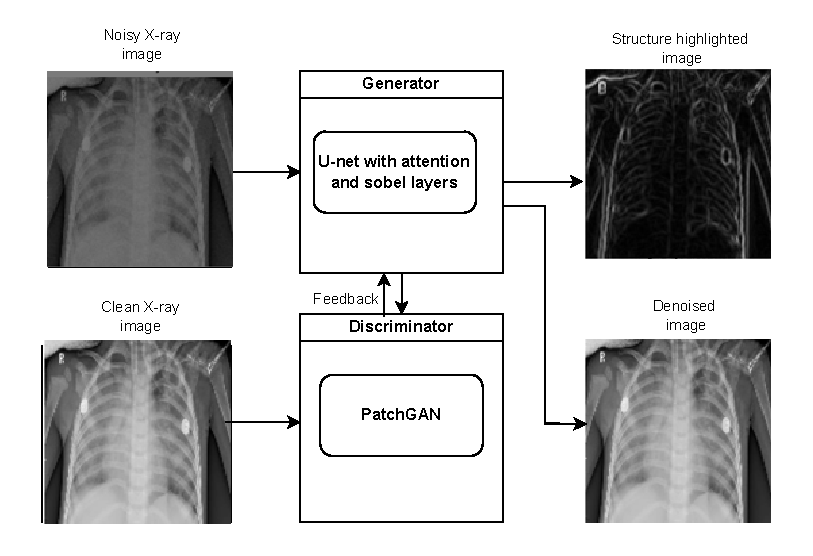
\includegraphics[width=0.85\textwidth]{images/XGAN-block.pdf}
	\caption{Architecture of X-GAN. The generator uses a U-Net with an edge attention mechanism at the bottleneck. The discriminator uses a PatchGAN with spectral normalisation.}
	\label{fig:xgan_architecture}
\end{figure}

The generator uses a U-Net architecture. We added an edge attention mechanism at the bottleneck layer. This mechanism computes gradient information using a Sobel operator and uses it to create spatial and channel-wise attention maps. The discriminator uses a PatchGAN architecture with spectral normalisation to stabilise training.

The loss function combines three components:

\[
L_{\text{total}} = \alpha L_{\text{MAE}} + \beta L_{\text{Edge}} + \gamma L_{\text{SSIM}}
\]

We performed a sensitivity analysis to find the optimal weights. The best performance occurred at \(\alpha = 1\), \(\beta = 5\), \(\gamma = 2\).

We trained and evaluated X-GAN on the Mendeley chest X-ray dataset \citep{sait2020curated}. This dataset contains 9,208 posterior-anterior chest X-ray images. We split the data into 80\% for training, 10\% for validation, and 10\% for testing. Since clean X-ray images are naturally noise-free, we simulated low-dose acquisitions by adding Poisson noise to the clean images. The noise level was controlled by a peak photon parameter set to \(\lambda = 1000\). All images were resized to \(256 \times 256\) pixels and normalised to the range \([0,1]\).

\subsection{Results}

Table~\ref{tab:xgan} compares X-GAN with state-of-the-art methods.

\begin{table}[H]
	\centering
	\caption{Performance comparison on chest X-ray denoising}
	\label{tab:xgan}
	\begin{tabular}{lcccc}
		\toprule
		Model & PSNR (dB) & SSIM & EPI & Parameters (M) \\
		\midrule
		RIDNet & 34.80 & 0.89 & 0.547 & 1.79 \\
		CBDNet & 34.44 & 0.89 & 0.561 & 4.57 \\
		X-ReCNN & 35.53 & 0.94 & 0.579 & 0.09 \\
		CGAN & 30.21 & 0.79 & 0.347 & 179.88 \\
		\textbf{X-GAN} & \textbf{36.48} & \textbf{0.95} & \textbf{0.721} & \textbf{2.17} \\
		\bottomrule
	\end{tabular}
\end{table}

X-GAN achieves the highest PSNR, SSIM, and EPI. It has 98\% fewer parameters than a standard CGAN.

\subsubsection{Ablation study}

We performed a component-wise ablation study to isolate the contribution of each design choice. Table~\ref{tab:xgan_ablation} shows the progressive improvement.

\begin{table}[H]
	\centering
	\caption{Component-wise ablation study}
	\label{tab:xgan_ablation}
	\begin{tabular}{lcccc}
		\toprule
		Configuration & PSNR & SSIM & E.RMSE & EPI \\
		\midrule
		U-Net + MAE & 33.20 & 0.92 & 0.12 & 0.35 \\
		+ Hybrid Loss & 35.70 & 0.94 & 0.09 & 0.47 \\
		+ Edge Attention & 35.84 & 0.94 & 0.06 & 0.62 \\
		+ \(4 \times 4\) Kernels & 36.48 & 0.95 & 0.05 & 0.71 \\
		\bottomrule
	\end{tabular}
\end{table}

The hybrid loss gave the largest improvement in PSNR (2.5 dB). Adding edge attention improved EPI from 0.47 to 0.62, confirming that the attention mechanism specifically helps preserve edges. The larger kernels provided a final boost in both PSNR and EPI.

\subsubsection{Downstream classification}

To evaluate clinical utility, we used X-GAN as a preprocessing step for a diagnostic classifier. Table~\ref{tab:xgan_downstream} shows the classification performance.

\begin{table}[H]
	\centering
	\caption{Impact of X-GAN denoising on downstream classification}
	\label{tab:xgan_downstream}
	\begin{tabular}{lccc}
		\toprule
		Model & Input & Accuracy & F1-score \\
		\midrule
		VGG-16 & Noisy & 69.75\% & 0.636 \\
		VGG-16 & X-GAN denoised & 80.00\% & 0.796 \\
		ResNet-50 & Noisy & 54.55\% & 0.568 \\
		ResNet-50 & X-GAN denoised & 79.52\% & 0.718 \\
		EfficientNetV2 & Noisy & 72.75\% & 0.707 \\
		EfficientNetV2 & X-GAN denoised & 87.00\% & 0.860 \\
		\bottomrule
	\end{tabular}
\end{table}

Denoising with X-GAN improved classification accuracy across all three architectures. ResNet-50 showed the largest gain, from 54.55\% to 79.52\%. EfficientNetV2 achieved the highest overall accuracy of 87.00\% on denoised images.

\subsubsection{Clinical evaluation}

We conducted a blinded mean opinion score (MOS) study with two experienced radiologists. They rated 50 randomly selected images on a 5-point scale across four dimensions: noise suppression, texture preservation, artifact freedom, and diagnostic confidence. Table~\ref{tab:xgan_mos} shows the results.

\begin{table}[H]
	\centering
	\small
	\caption{Blinded MOS from two radiologists. Values are mean ± standard deviation on a 5-point scale. Higher is better for all metrics.}
	\label{tab:xgan_mos}
	\begin{tabular}{lcccc}
		\toprule
		Model & Noise Suppression & Texture Preservation & Artifact Freedom & Diagnostic Conf. \\
		\midrule
		Noisy Input & 1.34 ± 0.51 & 4.92 ± 0.31 & 5.00 ± 0.00 & 2.20 ± 0.60 \\
		CBDNet & 4.04 ± 0.40 & 2.10 ± 0.50 & 4.02 ± 0.40 & 2.90 ± 0.50 \\
		RIDNet & 4.20 ± 0.49 & 2.98 ± 0.40 & 3.96 ± 0.40 & 3.30 ± 0.52 \\
		CGAN & 3.40 ± 0.71 & 3.00 ± 0.80 & 1.90 ± 0.59 & 2.40 ± 0.71 \\
		X-ReCNN & 4.90 ± 0.30 & 3.10 ± 0.50 & 4.60 ± 0.49 & 3.96 ± 0.40 \\
		\textbf{X-GAN} & \textbf{4.84 ± 0.36} & \textbf{4.70 ± 0.46} & \textbf{4.90 ± 0.30} & \textbf{4.90 ± 0.25} \\
		\bottomrule
	\end{tabular}
\end{table}

X-GAN achieved the highest diagnostic confidence score (4.90 ± 0.25), outperforming X-ReCNN (3.96 ± 0.40). It also scored highest in texture preservation (4.70 ± 0.46) and artifact freedom (4.90 ± 0.30). The noisy input scored low on noise suppression (1.34) but high on texture preservation (4.92) – this is expected because noise has not been removed. X-GAN successfully removes noise while keeping the natural texture intact.

\subsection{Conclusion of phase I}

X-GAN denoises chest X-rays while preserving edges. The hybrid loss function and edge attention mechanism work together to prevent over-smoothing. The ablation study confirms that each component contributes to the final performance. The downstream classification experiment shows that denoising improves diagnostic accuracy. The model has 2.17 million parameters, making it suitable for clinical deployment.

% chapters/proposal-phase2.tex
% Replace the content below with your own text.

\section{Work Completed – Phase II: SAGA}
\label{sec:saga}
\subsection{Objective}

We proposed a spatially adaptive AF called SAGA. Unlike ReLU, which applies the same operation everywhere, SAGA uses local context to decide how to transform each pixel. We validated SAGA on two distinct medical imaging modalities: chest CT (soft tissue, continuous structures) and osteoporosis X-ray (sparse, high-frequency trabecular bone).

\subsection{Methodology}

Figure~\ref{fig:saga_methodology} provides an overview of the seven phases of our experimental framework.

\begin{figure}[H]
	\centering
	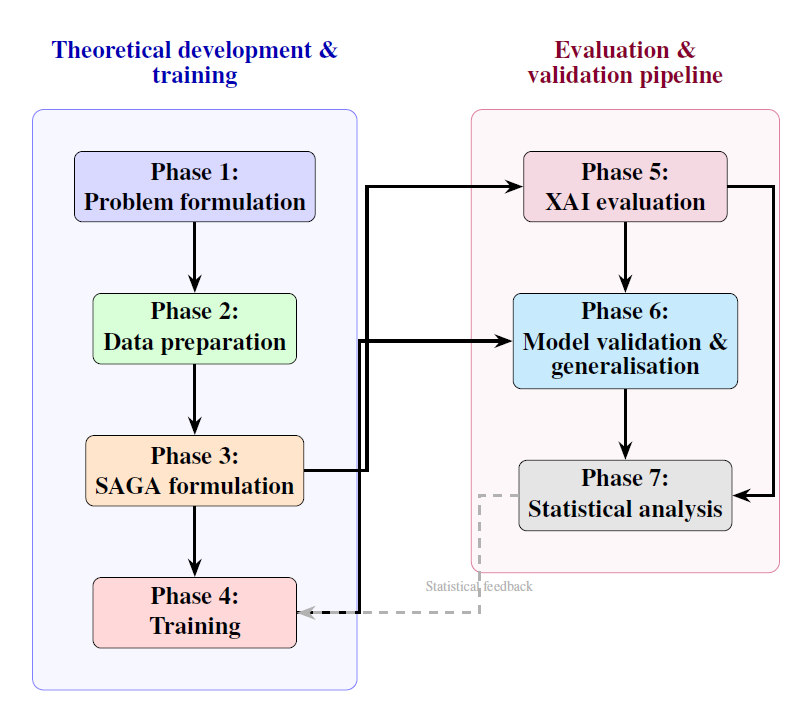
\includegraphics[width=0.85\textwidth]{SAGA-methodology.png}
	\caption{Seven-phase methodology of the SAGA framework. Phases 1-4 cover theoretical development and training. Phases 5-7 cover evaluation and validation.}
	\label{fig:saga_methodology}
\end{figure}

The core of our contribution is the SAGA operator. For an input feature map \(F\), SAGA performs three operations.

First, it extracts spatial context using a depthwise convolution followed by batch normalisation:

\[
T(F) = \text{BN}(\text{Conv}_{3\times3}^{\text{DW}}(F))
\]

Second, it computes a learnable gate using a pointwise convolution and a sigmoid function:

\[
G(F) = \sigma(\text{Conv}_{1\times1}(T(F)))
\]

Third, it combines the original feature map with a gated sharpening signal:

\[
\phi_{\text{SAGA}}(F) = F + G(F) \odot \text{ReLU}(T(F) - F)
\]

We proved several theoretical properties of SAGA, including non-saturation, gradient stability, and spatial adaptation.
We evaluated SAGA on two public medical imaging datasets. The first was a large-scale CT dataset \citep{syed2024medical} containing 1,000 high-resolution chest CT scans. The second was an osteoporosis X-ray dataset \citep{wani2021knee} containing 1,000 dual-energy X-ray absorptiometry scans of the knee. For each modality, we split the data into 800 training, 100 validation, and 100 testing images. To simulate realistic acquisition artefacts, we applied three types of degradation: Gaussian blur (\(\sigma = 1.0\) to \(5.0\)), motion blur (kernel sizes 9, 15, and 21), and defocus blur (disk radius 2 to 5 pixels). From each degraded image, we extracted non-overlapping patches of size \(256 \times 256\) pixels. For training, we generated 4,000 patches. For validation and testing, we generated 500 patches each. We applied random rotations, horizontal flips, and contrast adjustments as data augmentation.

We used four network architectures: VGGNet, ResNet, U-Net, and EDSR. We compared SAGA against six existing AFs: Sigmoid, Tanh, ReLU, ELU, Swish, and FReLU.

\subsection{Results}

We evaluated SAGA on two distinct medical imaging modalities using the VGGNet architecture. VGGNet is the simplest architecture we tested – it has no residual connections, no skip connections, and no attention mechanisms. Any improvement in deblurring quality must therefore come from the AF itself, not from architectural features compensating for a weak activation.

The chest CT dataset represents soft tissue with continuous anatomical structures. The osteoporosis X-ray dataset represents sparse, high-frequency trabecular bone against a dark background. This is a more challenging task because standard AFs often smooth these fine bone details, producing a waxy appearance that erases the trabecular mesh.

Table~\ref{tab:saga_comparison} compares SAGA against six existing AFs on both modalities using the VGGNet architecture.

\begin{table}[H]
	\centering
	\caption{Performance comparison of AFs on chest CT and osteoporosis X-ray deblurring using the VGGNet architecture. Values are PSNR (dB) and SSIM.}
	\label{tab:saga_comparison}
	\begin{tabular}{lcccc}
		\toprule
		\multirow{2}{*}{AF} & \multicolumn{2}{c}{Chest CT} & \multicolumn{2}{c}{Osteoporosis X-ray} \\
		\cline{2-5}
		& PSNR & SSIM & PSNR & SSIM \\
		\midrule
		Sigmoid & 26.45 & 0.74 & 35.82 & 0.88 \\
		Tanh & 30.91 & 0.84 & 35.81 & 0.87 \\
		ReLU & 26.45 & 0.73 & 36.13 & 0.88 \\
		ELU & 31.35 & 0.85 & 44.56 & 0.90 \\
		Swish & 26.44 & 0.74 & 36.02 & 0.88 \\
		FReLU & 35.60 & 0.93 & 44.84 & 0.95 \\
		\textbf{SAGA} & \textbf{37.16} & \textbf{0.96} & \textbf{50.33} & \textbf{0.98} \\
		\bottomrule
	\end{tabular}
\end{table}

On the chest CT dataset, SAGA achieves 37.16 dB PSNR and 0.96 SSIM, outperforming the next best method FReLU by 1.56 dB. On the more challenging osteoporosis dataset, the improvement is even larger. SAGA reaches 50.33 dB PSNR and 0.98 SSIM, which is 5.49 dB higher than FReLU and 14.2 dB higher than ReLU.

These results are particularly significant because they were obtained using VGGNet, the simplest architecture in our evaluation. Since VGGNet has no residual connections or skip connections to compensate for a weak AF, the improvement must come from SAGA's design itself. The spatial gating mechanism successfully distinguishes between diagnostically relevant edges and noise, even in sparse bone structures where other activations fail.

We also validated SAGA on three additional architectures – ResNet, U-Net, and EDSR – and observed consistent improvements across all of them. The complete results are reported in our published paper \citep{siju2026saga}. The average improvement of SAGA over ReLU across all four architectures and both modalities was 6.3 dB in PSNR and 0.09 in SSIM.

\subsubsection{Summary across architectures and modalities}

While the VGGNet results isolate the effect of the AF itself, we also validated SAGA on three additional architectures: ResNet, U-Net, and EDSR. Table~\ref{tab:saga_summary} summarises the performance across all four architectures and both datasets.

\begin{table}[H]
	\centering
	\caption{Summary of SAGA performance across architectures and modalities. Values are PSNR (dB) with SSIM in parentheses. The best baseline AF for each configuration is shown in brackets.}
	\label{tab:saga_summary}
	\begin{tabular}{lcccc}
		\toprule
		\multirow{2}{*}{Architecture} & \multicolumn{2}{c}{Chest CT} & \multicolumn{2}{c}{Osteoporosis} \\
		\cline{2-5}
		& Best Baseline & SAGA & Best Baseline & SAGA \\
		\midrule
		VGGNet & 35.60 (0.93) [FReLU] & \textbf{37.16 (0.96)} & 44.84 (0.95) [FReLU] & \textbf{50.33 (0.98)} \\
		ResNet & 31.39 (0.85) [ReLU] & \textbf{34.93 (0.93)} & 46.79 (0.95) [ReLU] & \textbf{48.82 (0.97)} \\
		U-Net & 34.01 (0.90) [FReLU] & \textbf{36.33 (0.95)} & 42.21 (0.92) [FReLU] & \textbf{44.86 (0.94)} \\
		EDSR & 34.43 (0.91) [FReLU] & \textbf{38.05 (0.96)} & 43.72 (0.91) [ReLU] & \textbf{47.97 (0.97)} \\
		\bottomrule
	\end{tabular}
\end{table}

Across all four architectures and both modalities, SAGA consistently outperforms the best baseline AF in every configuration. The average improvement over ReLU across all experiments was 6.3 dB in PSNR and 0.09 in SSIM. The improvement is largest on the challenging osteoporosis dataset, where fine trabecular details are easily lost. This confirms that SAGA's spatial gating mechanism generalises across architectures, from simple plain networks (VGGNet) to deep residual networks (ResNet, EDSR) and encoder-decoder structures (U-Net).

\subsubsection{Interpretability analysis}

We performed an interpretability analysis using layer-wise relevance propagation (LRP) \citep{montavon2018methods} and K-path visualisation \citep{bhati2025neural} on the ResNet backbone.

LRP decomposes the network's prediction into pixel-wise relevance scores. The Edge Concentration Score (ECS) measures how tightly these relevance scores are focused on anatomical boundaries. A higher ECS indicates that the network is paying attention to diagnostically relevant structures rather than scattering attention across the image.

After identifying the most important neurons using the GetOptimiser algorithm \citep{bhati2025neural}, we reconstructed the output using only these selected pathways. The Reconstruction MSE measures pixel-wise error between the full model output and the sparse reconstruction. The Reconstruction  Symmetric Mean Absolute Percentage Error (SMAPE) measures relative error as a percentage. Lower values in both metrics indicate that the selected neurons faithfully preserve the original prediction – meaning the network has efficient, non-redundant internal representations.

Table~\ref{tab:saga_lrp} compares these metrics across ReLU, FReLU, and SAGA.

\begin{table}[H]
	\centering
	\caption{LRP-based interpretability metrics. ECS measures spatial focus (higher is better). Reconstruction MSE and SMAPE measure how faithfully the selected neurons preserve the output (lower is better).}
	\label{tab:saga_lrp}
	\begin{tabular}{lccc}
		\toprule
		Metric & ReLU & FReLU & SAGA \\
		\midrule
		Edge Concentration Score (ECS) ↑ & 0.2279 & 0.2345 & \textbf{0.2506} \\
		Reconstruction MSE ↓ & 0.0186 & 0.0161 & \textbf{0.0130} \\
		Reconstruction SMAPE ↓ & 28.25\% & 28.84\% & \textbf{24.96\%} \\
		\bottomrule
	\end{tabular}
\end{table}

SAGA achieves a significantly higher ECS than both ReLU (\(p = 0.0298\)) and FReLU (\(p = 0.037\)). This means SAGA focuses network attention on diagnostically relevant boundaries such as the pleural wall and central vessels, rather than scattering attention across the image.

Despite operating at the same sparsity level (approximately 26\% of neurons active), SAGA's selected pathways reconstruct the output with 30.1\% lower MSE than ReLU and 19.3\% lower MSE than FReLU. The SMAPE values confirm this improvement: SAGA achieves 24.96\% relative error, compared to 28.25\% for ReLU and 28.84\% for FReLU. This indicates that SAGA packs more diagnostic information into each active neuron – its internal representations are more efficient and less redundant than those of baseline AFs.

Figure~\ref{fig:saga_lrp_kpath} visualises the LRP heatmaps and K-path activations for all three AFs.
The visualisation confirms the quantitative findings. ReLU produces scattered, diffuse relevance maps, indicating poor anatomical focus. FReLU improves slightly but exhibits isolated pixel hotspots due to its hard thresholding operation – a phenomenon called the absolute sparsity bottleneck. SAGA, in contrast, generates continuous edge-focused relevance along the pleural wall and central vessels. The K-path visualisations further reveal that SAGA achieves genuine feature disentanglement: distinct pathways specialise in texture extraction, boundary detection, and background suppression. ReLU and FReLU, by comparison, show redundant or disjointed activation patterns.
\begin{figure}[H]
	\centering
	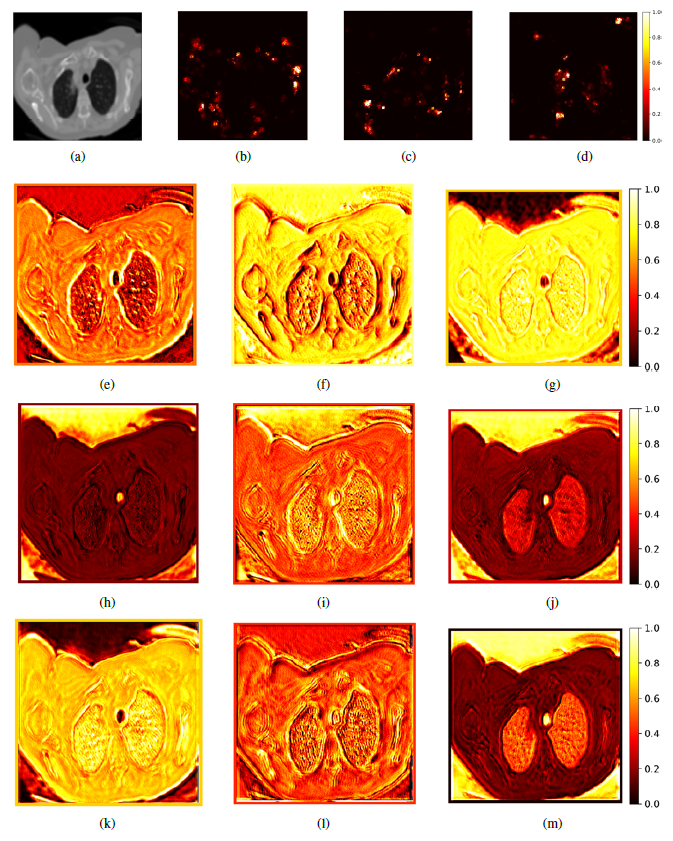
\includegraphics[width=0.9\textwidth]{SAGA-LRP-Kpath.png}
	\caption{LRP and K-Path analysis comparing AFs. (a) Input CT image. (b-d) LRP heatmaps: (b) ReLU, (c) FReLU, (d) SAGA. (e-m) Top-3 K-Path visualisations for (e-g) ReLU, (h-j) FReLU, and (k-m) SAGA. SAGA produces continuous edge-focused relevance (d) with spatially separated pathways (k-m), unlike the diffuse ReLU (b,e-g) and sparse FReLU (c,h-j) patterns.}
	\label{fig:saga_lrp_kpath}
\end{figure}



\subsection{Conclusion of phase II}

SAGA is a spatially adaptive AF that can be added to existing architectures without other changes. On the osteoporosis dataset, SAGA achieved 50.33 dB PSNR and 0.98 SSIM using VGGNet – 14.2 dB higher than ReLU. Across all four architectures and both modalities, the average improvement over ReLU was 6.3 dB in PSNR and 0.09 in SSIM. LRP analysis showed that SAGA's active neurons carry more useful information than ReLU (30.1\% lower reconstruction MSE at the same sparsity level). These results show that designing better AFs is an alternative to making networks deeper.

% chapters/proposal-phase3.tex
% Replace the content below with your own text.

\section{Remaining Work – Phase III}
\label{sec:phase3}
\subsection{Overview}

Phase III has two components. The first is Viveka, a test-time refinement framework that applies physics-based constraints directly to denoised images. The second is a Sobolev-regularised loss function called ADL\(_1\) with an attention-guided U-Net architecture called AG-UNet. Both components have been designed in detail. Preliminary experiments have been conducted. Manuscripts are in preparation.

\subsection{Phase III-A: Viveka – test-time refinement}

\subsubsection{Motivation}

Even physics-informed models like X-GAN are trained to minimise average error over a dataset. A model that works well on average may still produce visible artefacts on a specific patient image. Viveka addresses this by applying additional constraints at test time, without modifying the network weights.

\subsubsection{Methodology}

Viveka performs a single-pass deterministic refinement in four steps.

First, it decomposes the image into three anatomical zones based on X-ray attenuation coefficients: bone, lung, and background. Bone receives strong edge enhancement. Lung receives moderate enhancement. Background receives no enhancement.

Second, it extracts fine details using blockwise discrete cosine transform (DCT) filtering. It retains coefficients that exceed physics-informed thresholds. Cycle spinning reduces blocking artefacts.

Third, it computes an edge protection map that identifies anatomical boundaries. It also computes an uncertainty map that identifies regions where the base denoiser may have introduced artefacts.

Fourth, it fuses the base denoiser output with the DCT-extracted details using a weight map that combines anatomical zones, adaptive gains, edge protection, and uncertainty guidance.

\subsubsection{Preliminary results}

We evaluated Viveka on 50 genuinely noisy chest X-rays from the CheXpert dataset. We tested it with five base denoisers: X-GAN, RIDNet, CBDNet, X-ReCNN, and CGAN.

For over-smoothed models such as RIDNet, Viveka reduced NIQE from 25.25 to 6.38, a 75\% improvement. It restored edge density from 0.008 to 0.150. It recovered GLCM entropy from zero to 5.84, which is within 5\% of the noisy reference value of 5.77.

Viveka processes a \(256 \times 256\) image in 0.6 to 0.9 seconds on a standard CPU. It does not require a GPU. It produces interpretable difference maps that show exactly where the image was enhanced (blue) and where noise was suppressed (red).
\subsection{Phase III-B: ADL1 loss and AG-UNet}

\subsubsection{Motivation}

Standard loss functions such as MAE minimise pixel-wise error but provide no control over gradients. We proved mathematically that for any small pixel error, there exist images with arbitrarily large gradient errors. We call this the Sobolev Gap. The ADL\(_1\) loss closes this gap by explicitly penalising gradient errors.

\subsubsection{Theoretical foundation}

\textbf{Theorem 1 (Sobolev gap):} For any \(\epsilon > 0\), there exist perturbations \(\hat{Y}_\epsilon\) such that:

\[
\|\hat{Y}_\epsilon - Y\|_{L^1} < \epsilon \quad \text{but} \quad \|\nabla \hat{Y}_\epsilon - \nabla Y\|_{L^1} > \frac{1}{\epsilon}
\]

This means that a network can achieve arbitrarily low MAE while having arbitrarily large edge errors.

\textbf{Theorem 2 (Gradient convergence):} If the ADL\(_1\) loss is small, then the gradients of the prediction are close to the gradients of the ground truth. Formally, minimising ADL\(_1\) guarantees convergence in the Sobolev space \(W^{1,1}\).

The ADL\(_1\) loss is defined as:

\[
\mathcal{L}_{\text{ADL1}}(\hat{Y},Y) = \mathbb{E}\left[\|\hat{Y} - Y\|_1 + \lambda_G \sum_{s=1}^{S} w_s \| \mathcal{G}_s(\hat{Y}) - \mathcal{G}_s(Y) \|_1\right]
\]

where \(\mathcal{G}_s\) computes gradients at multiple scales.

\subsubsection{Architecture: AG-UNet}

The Attention-Guided U-Net (AG-UNet) modifies standard U-Net in two ways.

First, it replaces standard skip connections with Edge-Weighted Channel Attention (EWCA) modules. These modules use the gradient of the input image as a spatial gate. They filter out background noise before features reach the decoder.

Second, it replaces standard convolutional layers with Multi-Scale Feature Blocks (MSFB) that use parallel dilated convolutions to capture context at multiple scales.

\subsubsection{Preliminary results}

We evaluated the ADL\(_1\) loss and AG-UNet on chest CT and osteoporosis X-ray datasets.

Table~\ref{tab:adl1} shows the impact of the loss function on the simple U-Net architecture.

\begin{table}[H]
	\centering
	\caption{Impact of loss function on edge preservation (EPI)}
	\label{tab:adl1}
	\begin{tabular}{lcc}
		\toprule
		Loss Function & CT EPI & Bone EPI \\
		\midrule
		MAE & 0.121 & 0.121 \\
		ADL\(_1\) & 0.659 & 0.210 \\
		\bottomrule
	\end{tabular}
\end{table}

Using ADL\(_1\) improves EPI by a factor of five on CT data and nearly doubles it on bone data.

Table~\ref{tab:agunet} compares AG-UNet with baseline architectures.

\begin{table}[H]
	\centering
	\caption{Architecture comparison on osteoporosis dataset}
	\label{tab:agunet}
	\begin{tabular}{lccc}
		\toprule
		Model & PSNR (dB) & EPI & FID \\
		\midrule
		U-Net & 38.12 & 0.120 & 66.21 \\
		Attention U-Net & 38.77 & 0.143 & 68.40 \\
		EDSR & 40.10 & 0.212 & 35.48 \\
		\textbf{AG-UNet} & 39.96 & \textbf{0.370} & \textbf{20.42} \\
		\bottomrule
	\end{tabular}
\end{table}

EDSR achieves the highest PSNR by aggressively smoothing the background. But its EPI is low, meaning it loses fine trabecular details. AG-UNet achieves 74.5\% higher EPI and 42\% lower FID, indicating better preservation of bone structure.

\subsection{Expected outcomes of phase III}

We expect Viveka to provide a model-agnostic test-time refinement that works with any denoiser. It will be fast, interpretable, and require no retraining.

We expect the ADL\(_1\) loss and AG-UNet to provide a mathematically grounded framework for deblurring that guarantees edge preservation. The Sobolev regularisation will prevent the smoothing artefacts that plague standard pixel-wise losses.

\subsection{Publication plan}

Manuscripts describing Viveka and the ADL\(_1\)/AG-UNet framework are in preparation. We plan to submit Viveka to \textit{Medical Image Analysis} or \textit{IEEE Transactions on Medical Imaging}. We plan to submit ADL\(_1\)/AG-UNet to \textit{IEEE Transactions on Pattern Analysis and Machine Intelligence} or \textit{IEEE Transactions on Image Processing}.


% chapters/proposal-contributions.tex
% Replace the content below with your own text.

\section{Expected Contributions to the Field}
\label{sec:ec}
\subsection{Theoretical contributions}

We have proved the existence of the Sobolev Gap in medical image restoration, showing that pixel-wise losses cannot guarantee edge preservation. We have formulated the ADL\(_1\) loss that closes this gap and guarantees convergence in Sobolev space. We have proved that SAGA has desirable properties including non-saturation, gradient stability, and spatial adaptation.

\subsection{Architectural contributions}

X-GAN is a lightweight physics-informed GAN for chest X-ray denoising with only 2.17 million parameters. SAGA is a drop-in AF that improves deblurring performance across multiple architectures. AG-UNet introduces gradient-guided attention for edge-preserving restoration.

\subsection{Practical contributions}

X-GAN improves downstream classification accuracy from 54.55\% to 79.52\%, demonstrating clinical utility. SAGA improves PSNR by 6.3 dB on average over ReLU. Viveka processes images in under one second on a CPU and produces interpretable difference maps. The ADL\(_1\) loss prevents the waxy smoothing that makes standard denoisers clinically unacceptable.

\subsection{Social contribution}

By enabling effective denoising at lower radiation doses, this research can reduce patient exposure to X-rays. By preserving fine anatomical details, it can improve diagnostic accuracy for conditions such as osteoporosis and lung nodules. By providing interpretable outputs, it can build trust between clinicians and AI systems.

% chapters/proposal-publications.tex
% Replace the content below with your own text.

\section{List of Publications}
\label{sec:pub}
\subsection{Published journal articles}

\begin{enumerate}
	\item Siju K.S., Venugopal V., Sowmya V., Mithun Kumar Kar. X-GAN: Physics-informed generative model for edge-preserved chest X-ray image denoising. \textit{Computer Methods and Programs in Biomedicine Update}, 9:100247, 2026.~\url{https://doi.org/10.1016/j.cmpbup.2026.100247}.
	\item Siju K.S., Venugopal V., Mithun Kumar Kar., Anandakrishnan J. An interpretable deep learning method for medical image deblurring and restoration using Spatially Adaptive Gated Activation (SAGA). \textit{Healthcare Analytics}, 9:100468, 2026.~\url{https://doi.org/10.1016/j.health.2026.100468}.
\end{enumerate}

\subsection{Manuscripts in preparation}

\begin{enumerate}
	\item Siju K.S., Venugopal V., Mithun Kumar Kar. Viveka: A test-time physics-aware refinement framework for chest X-ray denoising. Target: \textit{Medical Image Analysis} or \textit{IEEE Transactions on Medical Imaging}.
	\item Siju K.S., Venugopal V., Mithun Kumar Kar. Bridging the Sobolev Gap: Augmented Differential L\(_1\) loss for structure-preserving medical image deblurring. Target: \textit{IEEE Transactions on Pattern Analysis and Machine Intelligence} or \textit{IEEE Transactions on Image Processing}.
\end{enumerate}

% chapters/proposal-timeline.tex
% Replace the content below with your own text.

\section{Ph.D. Programme Completion Plan}
\label{sec:cp}
\begin{table}[H]
	\centering
	\caption{Completion plan}
	\label{tab:plan}
	\begin{tabular}{lp{3cm}p{6cm}}
		\toprule
		Milestone & Planned Date & Status \\
		\midrule
		Course work & January 2025 & Completed \\
		Comprehensive examination & December 2025 & Completed \\
		Phase I publication (X-GAN) & June 2026 & Published \\
		Phase II publication (SAGA) & June 2026 & Published \\
		Qualifying examination& July 2026&Planned\\
		Phase III-A implementation & July–September 2026 & In progress \\
		Phase III-B implementation & October–December 2026 & In progress \\
		Open Seminar I & August 2026 & Planned \\
		Phase III-A manuscript submission & August 2026 & Planned \\
		Phase III-B manuscript submission & September 2026 & Planned \\
		Open Seminar II & February 2027 & Planned \\
		Synopsis submission & March 2027 & Planned, subject to the completion of seminars \\
		Thesis submission & May 2027 & Final milestone, planned \\
		\bottomrule
	\end{tabular}
\end{table}

% ---- BIBLIOGRAPHY ------------------------------------------
\newpage
\bibliography{references}

\end{document}
